\documentclass[11pt]{article}
\usepackage[margin=1in]{geometry}
\usepackage[utf8]{inputenc}
\usepackage[english]{babel}
\usepackage[T1]{fontenc}
\usepackage{fourier}
\usepackage{amsthm}
\usepackage{amssymb}
\usepackage{amsmath}
\usepackage{amsfonts}
\usepackage{latexsym}
\usepackage{graphicx}
\usepackage{float}
\usepackage{etoolbox}
\usepackage{hyperref}
\usepackage{tikz}
\usepackage{lipsum}
\usepackage{algorithm}
\usepackage{algpseudocode}
\usepackage{mathtools}
\usepackage{nccmath}

% add counters for theorems, definutions, remarks, etc. In italian
\newtheorem{teorema}{Teorema}[section]
\newtheorem{definuzione}[teorema]{Definuzione}
\newtheorem{osservazione}[teorema]{Osservazione}
\newtheorem{esempio}[teorema]{Esempio}
\newtheorem{proposizione}[teorema]{Proposizione}
\newtheorem{corollario}[teorema]{Corollario}
\newtheorem{lemma}[teorema]{Lemma}
\newtheorem{esercizio}[teorema]{Esercizio}

\newcommand{\R}{\mathbb{R}}
\newcommand{\N}{\mathbb{N}}
\newcommand{\Z}{\mathbb{Z}}
\newcommand{\Q}{\mathbb{Q}}
\newcommand{\C}{\mathbb{C}}

\title{Queueing System with Potential for Recruiting Secondary Servers}
\author{Luca Lombardo}
\date{}

\begin{document}
\maketitle
\tableofcontents

\section{Introduzione}



\subsection{Queueing Theory}

% Queueing models are used to represent systems of resources, traditionally called “servers”, which are to be used by several users, called “customers”. The terminology stems from applications like bank tellers, hotel reception desks, toll booths on freeways, and so on, where customers actually queue up until they are served by an employee. Queueing theory is used in much more diverse circumstances, however. \\

% \noindent Simple queues consist of one server which attends to one customer at a time, in order of their arrivals, with the added assumption that customers are indefinutely patient. We assume that time is discretized into intervals of fixed length, that a random number of customers join the system during each interval, and that the server removes one customer from the queue at the end of each interval,if there is any. Definung $\alpha_n$ as the number of new arrivals during the interval
% $[n - 1, n)$ and $X_n$ as the number of customers in the system at time $n$, we have

% \begin{equation}
%     \begin{cases}
%         X_n + \alpha_{n+1} - 1 & \text{if } X_n + \alpha_{n+1} \geq 1 \\
%         0 & \text{if } X_n + \alpha_{n+1} = 0
%     \end{cases}
% \end{equation}

% \noindent If $\{\alpha_n \}$ is a collection of independent random variables, then $X_{n+1}$ is conditionally independent of $X_0 , . . . , X_{n-1}$ if $X_n$ is known. If, in addition, the $\alpha_n$'s are identically distributed, then ${X_n}$ is homogeneous. The state space is $\N$.

I modelli di coda sono utilizzati per rappresentare sistemi di risorse, tradizionalmente chiamati "server", che devono essere utilizzati da diversi utenti, chiamati "clienti". La terminologia deriva da applicazionu come gli sportelli bancari, le reception degli hotel, i caselli autostradali, e così via, dove i clienti effettivamente si mettono in coda finché non vengono serviti da un dipendente. Tuttavia, la teoria delle code viene utilizzata in contesti molto più diversi. \vspace*{0.4cm}

\noindent Le code semplici consistono di un solo server che attende un solo cliente alla volta, in ordine di arrivo, con l'aggiunta dell'assunzione che i clienti siano indefinutamente pazienti. Si assume che il tempo sia discretizzato in intervalli di lunghezza fissa, che un numero casuale di clienti si unusca al sistema durante ognu intervallo e che il server rimuova un cliente dalla coda alla fine di ognu intervallo, se presente. Definendo $\alpha_n$ come il numero di nuovi arrivi durante l'intervallo $[n - 1, n)$ e $X_n$ come il numero di clienti nel sistema al tempo $n$, abbiamo

\begin{equation}
    X_{n+1} =
    \begin{cases}
        X_n + \alpha_{n+1} - 1 & \text{se } X_n + \alpha_{n+1} \geq 1 \\
        0 & \text{se } X_n + \alpha_{n+1} = 0
    \end{cases}
\end{equation}

\noindent Se ${\alpha_n}$ è una collezione di variabili casuali indipendenti, allora $X_{n+1}$ è condizionalmente indipendente da $X_0, \ldots, X_{n-1}$ se $X_n$ è noto. Se, inoltre, le $\alpha_n$ sono identicamente distribuite, allora ${X_n}$ è omogenea. Lo spazio degli stati è $\N$ e la matrice di transizione è

\begin{equation}
    P = \begin{pmatrix}
        q_0 + q_1 & q_2 & q_3 & q_4 & \ldots \\
        q_0 & q_1 & q_2 & q_3 & \ddots \\
        \vdots & q_0 & q_1 & q_2 & \ddots \\
        0 &  & \ddots & \ddots & \ddots
    \end{pmatrix}
\end{equation}

\noindent dove $q_i$ è la probabilità $P[\alpha=i]$ che $i$ nuovi clienti che entrino in coda durante un intervallo di un'unutà di tempo, mentre $\alpha$ denota ognuna delle possibili distribuzioni di $\alpha_n$ identicamente distribuite. Le catene di Markov aventi matrice di transizione della forma

\begin{equation}
    P = \begin{pmatrix}
        B1 & B_2 & B_3 & B_4 & \ldots \\
        A_0 & A_1 & A_2 & A_3 & \ddots \\
            & A_0 & A_1 & A_2 & \ddots \\
        0   &     & \ddots & \ddots & \ddots
    \end{pmatrix}
\end{equation}

\noindent dove $A_i, B_{i+1}, i \geq 0$ sono matrici non negative di dimensione $k \times k$ sono dette M/G/1-type Markov Chains e sono utilizzate per modellare svariati problemi di coda.

\subsection{Obiettivi del paper}

\noindent Il paper presenta un nuovo approccio per migliorare i modelli di coda con l'utilizzo di server secondari temporanei, reclutati tra i clienti stessi. Questi server secondari sono disponubili solo temporaneamente e fornuranno servizi in gruppi di diverse dimensionu. Dopo aver servito esattamente un gruppo, i server secondari lasceranno il sistema, permettendo ai clienti di proseguire le loro attività senza essere trattenuti. Il contributo principale del paper è l'introduzione del concetto di reclutamento di server secondari da parte dei clienti, in modo da aiutare il sistema. I risultati numerici indicano che il modello proposto funziona meglio del modello di coda classico corrispondente. Questo può aiutare i responsabili del sistema a reclutare server secondari quando necessario per migliorare le prestazionu del sistema. \\

\noindent Il paper analizza anche altri approcci di modelli di coda con server secondari presenti in letteratura. Tuttavia, andremo a considerare le due seguenti caratteristiche che sono intrinseche in alcunu sistemi del mondo reale e non sono state studiate in passato: (i) un server secondario verrà assegnato ad un gruppo (che non supererà una soglia finuta prestabilita); questo server offrirà i servizi uno alla volta; e una volta che tutti i clienti assegnati sono stati serviti, il server secondario lascerà anche il sistema; e (ii) con una certa probabilità, un cliente servito da un server secondario diventa insoddisfatto e quindi torna al sistema principale per ottenere un nuovo servizio.

\clearpage

\section{Modello Matematico}


Consideriamo un sistema di coda a singolo server in cui gli arrivi avvengono secondo un processo di arrivo markoviano (MAP) con matrici di parametro (D0, D1) di ordine m. Il MAP generalizza alcuni dei processi puntiformi ben noti come Poisson, Poisson interrotto e rinnovamenti di tipo fase, tra gli altri. Inoltre, MAP è ideale in situazioni in cui può essere presente una correlazione nei tempi tra gli arrivi. Supponiamo che gli arrivi provengano da diverse fonti in un'area comune per il trattamento. Anche se tutte le singole fonti generano arrivi secondo processi di rinnovo, quello combinato potrebbe non essere necessariamente un processo di rinnovo (a meno che tutte le singole fonti siano processi di Poisson). Un'altra parte attraente dell'uso di MAP è che l'analisi richiede il formalismo delle matrici e le ragioni intuitive associate all'analisi.

\subsection{Markovian arrival process (\textsc{map})}

Il generatore irriducibile del MAP è dato da $D_0 + D_1$. Sia $\delta$ il vettore invariante tale che
\begin{equation} \label{eq:invariant}
    \delta (D_0 + D_1) = \textbf{0}, \qquad \delta e = 1
\end{equation}
Dove d'ora in poi, $e$ è il vettore colonna di tutti gli elementi 1 con appropriata dimensione mentre $\textbf{0}$ rappresenta il vettore riga di tutti zeri con dimensioni appropriate. La matrice $D_0$ governa le transizionu corrispondenti al generatore sottostante che non produce arrivi, mentre la matrice  $D_1$ governa quelle transizioni corrispondenti agli arrivi nel sistema. \\

\noindent Il rate medio di arrivi $(\lambda)$, la varianza degli tempi internu di arrivo
$(\sigma^2)$ e la correlazione $(\rho_c)$ tra due successivi tempi internu di arrivo sono dati da

\begin{equation}
    \lambda = \delta D_1 e, \qquad \sigma^2 = \frac{2}{\lambda} \delta (-D_0)^{-1} e - \frac{1}{\lambda^2}, \qquad \rho_c = \frac{\lambda \delta (-D_0)^{-1} D_1 (-D_0)^{-1} e - 1}{2 \lambda \delta (-D_0)^{-1} e - 1}
\end{equation}
Il sistema ha un singolo server che offre servizi in modo FCFS. Questo server sarà chiamato server principale. I tempi di servizio sono esponenziali con parametro $\mu_1$. Con probabilità $p, 0 \leq p \leq 1$, un cliente servito può essere reclutato (o optato dal punto di vista del cliente servito) per servire altri clienti in attesa nel sistema (assumendo che la dimensione della coda sia positiva) a condizione che non ci sia già un altro server secondario che sta servendo. Un tale server è chiamato server secondario. In altre parole, una reclutamento avviene solo quando c'è almeno un cliente in attesa nella coda e quando non c'è altro server secondario presente nel sistema. Pertanto, il sistema può avere al massimo due server in qualsiasi momento. Si noti che con probabilità $q = 1 - p$, il cliente servito, che può diventare il server secondario, non accetta di farlo e lascia il sistema. Quando viene reclutato un server secondario, il server verrà assegnato a un gruppo di, diciamo, i clienti, dove $i = \min \{\text{numero nella coda}, L\}$, dove $L$ è un pre-determinato positivo finuto intero. In altre parole, $1 \leq L < \infty$. Il server secondario offrirà servizi ai clienti del gruppo uno alla volta e i tempi di servizio sono distribuiti in modo esponenziale con parametro $\mu_2$. Un cliente che riceve un servizio da un server secondario potrebbe non essere soddisfatto del servizio ricevuto e richiedere di essere servito di nuovo con probabilità $\nu$, $0 \leq \nu \leq 1$, e con probabilità $\bar \nu = 1 - \nu$ lascerà il sistema. I clienti insoddisfatti sono reinseriti nel sistema. Una volta che il server secondario ha finuto di servire tutti i clienti assegnati, il sistema rilascerà questo server.
Si noti che prendendo $p = 0$ (in questo caso $\nu$ non ha alcun ruolo e può essere ignorato), ottenuamo
il modello di coda a singolo server classico. Questo caso viene utilizzato solo come verifica dell'accuratezza nei calcoli numerici e non è altrimenti interessante. Il caso in cui $\nu = 1$ non è interessante poiché in questo caso ognu cliente servito da un server secondario viene reinserito nel sistema e l'assunzione di server secondari rallenta solo il sistema nell'offrire servizi.

\begin{figure}[h]
    \centering
    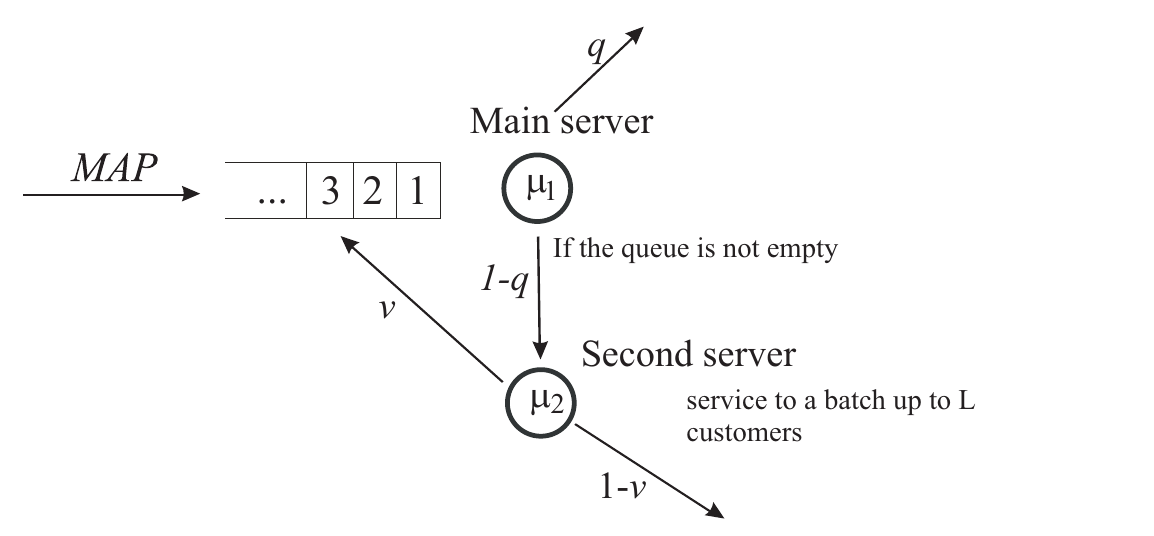
\includegraphics[width=0.8\textwidth]{hVQg024.png}
    \caption{Structure of the system under study}
    \label{fig:diagramma_di_stato}
\end{figure}

\section{\textsc{qbd} Approach to the Steady State Analysis}

Analizzeremo il modello di coda in studio in stato stazionario. L'analisi può essere effettuata tramite il processo QBD o tramite un tipo GI/M/1. In questa sezione, adotteremo l'approccio QBD, mentre nella prossima sezione evidenzieremo brevemente l'altro approccio. Come è noto, il processo QBD è un caso particolare della catena di Markov a tempo continuo (CTMC). \emph{Concetto dato per buono}

\subsection{Description of the QBD Process Governing the System and Its Generator}

Supponiamo che, al tempo $t\geq 0$, indichiamo:
\begin{itemize}
    \item il numero di clienti nel sistema come $i_t\geq 0$;
    \item il numero di clienti in servizio al server secondario come $n_t\in\{0,\ldots,\min(i_t,L)\}$ (notare che quando $n_t=0$, il sistema non ha un server secondario);
    \item lo stato del processo sottostante del MAP che descrive gli arrivi dei clienti come $\xi_t=1,\ldots,m$.
\end{itemize}
Allora, il processo stocastico $\{\zeta_t=(i_t,n_t,\xi_t),,t\geq 0\}$ che descrive il comportamento del modello in esame è un CTMC regolare e irriducibile. Enumerando gli stati del CTMC, $\{\zeta_t,,t\geq 0\}$, in ordine lessicografico e indicando con $i$ il livello, per $i\geq 0$, l'insieme di stati come $\{(i,n,k):0\leq n\leq \min(i,L),,1\leq k\leq m\}$, il generatore (infinitesimale), $Q$, di questo CTMC è dato dal seguente teorema.

\clearpage
\begin{teorema}
    Il generatore infinitesimale $Q$ del processo stocastico CTMC $\{\zeta_t,,t\geq 0\}$ ha una struttura a blocchi tridiagonale

    \begin{figure}[h]
        \centering
        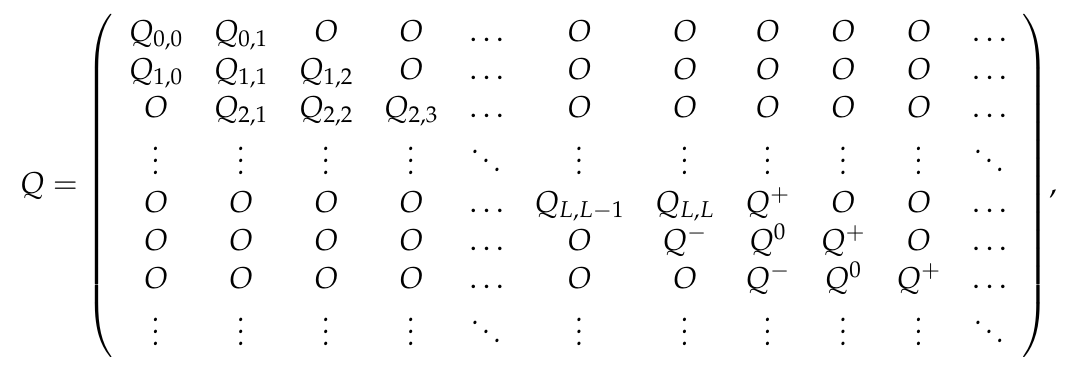
\includegraphics[width=0.6\textwidth]{E9pbGl1.png}
        \label{fig:generatore_infinitesimale}
    \end{figure}

    \noindent Dove i blocchi $Q_{i,i}$ non nulli sono definiti come segue

    \begin{figure}[h]
        \centering
        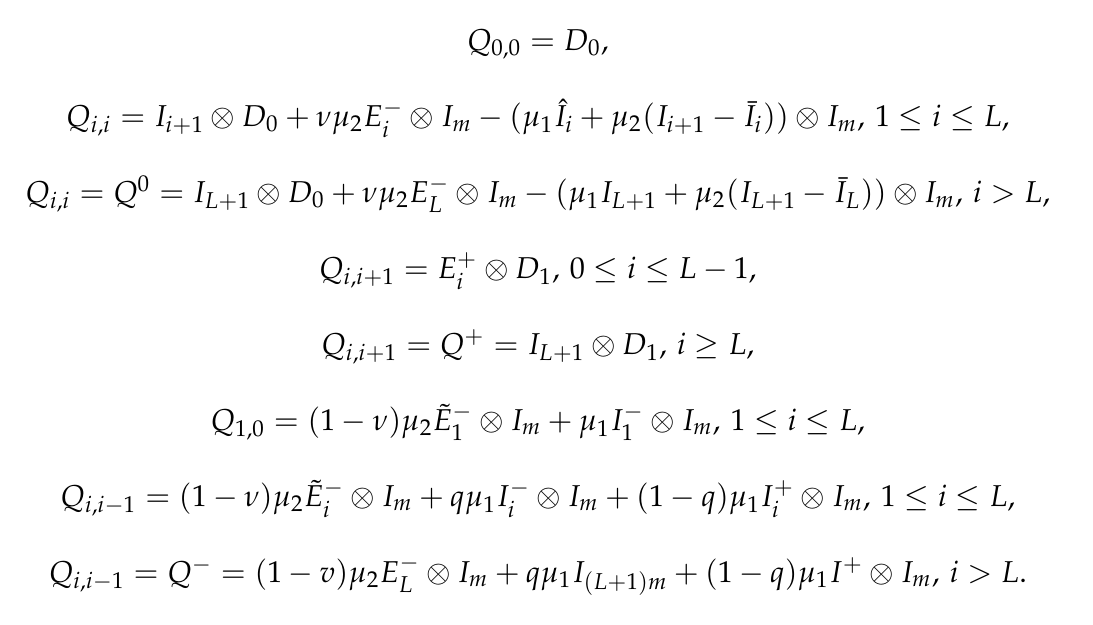
\includegraphics[width=0.6\textwidth]{T9RIVqa.png}
    \end{figure}

    \noindent Dove si usa la seguente notazione:

    \begin{figure}[h]
        \centering
        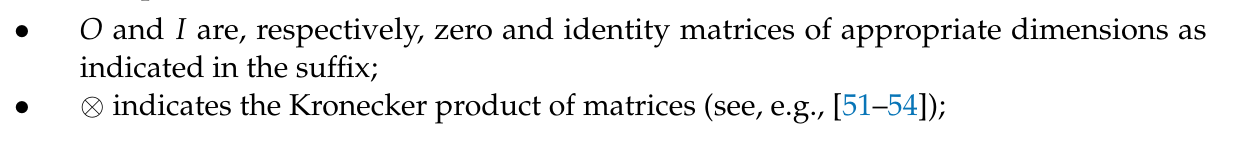
\includegraphics[width=0.8\textwidth]{avNOocE.png}
    \end{figure}

    \begin{figure}[h!]
        \centering
        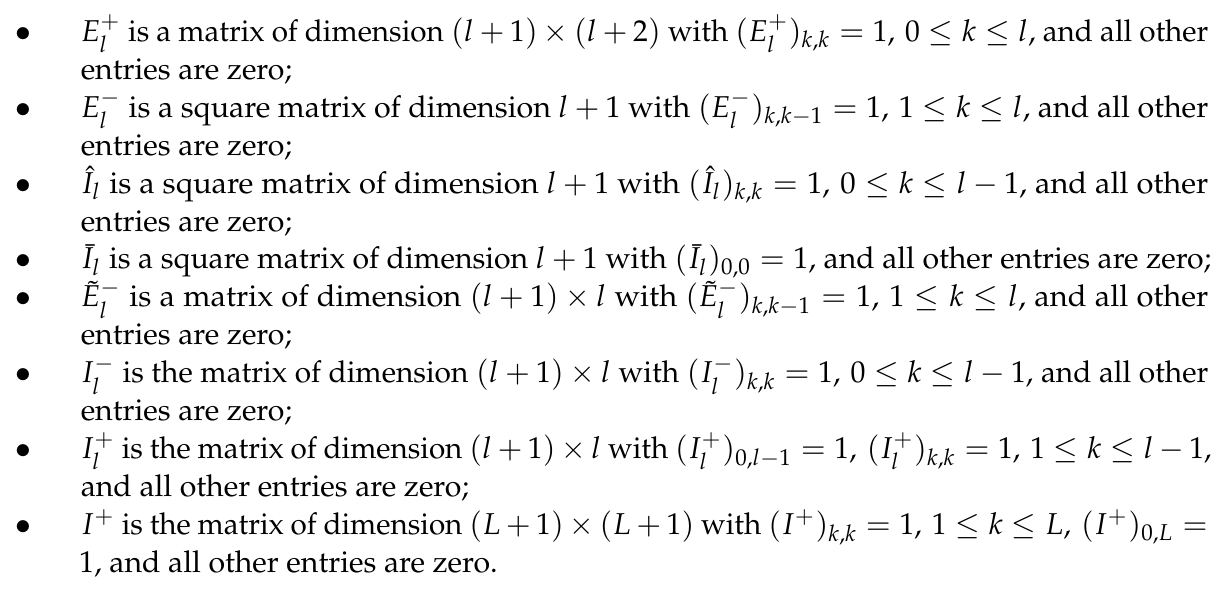
\includegraphics[width=0.8\textwidth]{px6kcg9.png}
    \end{figure}

    \begin{proof}
        Immediata
    \end{proof}

\end{teorema}
\clearpage

\subsection{Ergodicity Condition of the QBD Process}


\begin{teorema}
    Il processo stocastico CTMC $\{\zeta_t,,t\geq 0\}$ è ergodico se e solo se vale la seguente disuguaglianza:

    \begin{equation}\label{eq:ergodicity}
        \lambda < \mu_1 + \mu_2(1 - \nu) \frac{L(1-q)\mu_1}{L(1-q)\mu_1 + \mu_2}
    \end{equation}

    \begin{proof}
        È noto, grazie all'approccio matriciale-geometrico di Neuts (vedi, ad esempio, il riferimento [37]), che il criterio per l'ergodicità del QBD con il generatore di forma data in (3) è la soddisfazione dell'ineguaglianza:
        \begin{equation}\label{eq:ergodicity}
            y Q^- e > y Q^+e
        \end{equation}
        dove il vettore $y$ è l'unica soluzione del sistema
        \begin{equation}
            y(Q^- + Q^0 + Q^+) = \textbf{0}, \qquad ye = 1
        \end{equation}
        Si può inoltre verificare facilmente che
        \begin{equation}\label{eq:bigotimes}
            Q^- + Q^0 + Q^+ = I_{L+1} \bigotimes (D_0 + D_1) + S \bigotimes I_{m}
        \end{equation}
        dove
        \begin{figure}[h!]
            \centering
            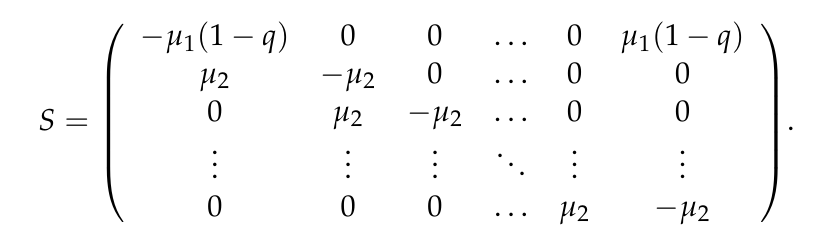
\includegraphics[width=0.6\textwidth]{lLnSEzP.png}
        \end{figure}
        Usando la regole del mixed product per il prodotto di Kronecker, ed usando \ref{eq:invariant} si verifica che la soluzione del sistema di equazioni lineari è
        \begin{equation}
            y = x \bigotimes \delta
        \end{equation}
        dove $\delta$ è come definita in \ref{eq:invariant} ed $x$ è la soluzione del sistema
        \begin{equation}\label{eq:system}
            xS = 0, \qquad xe = 1
        \end{equation}
        per sostituzione diretta, si verifica facilmente che le componenti del vettore $x = (x_0, x_1, ... , x_L)$, corrispondenti alle uniche soluzioni del sistema \ref{eq:system}, sono date da
        \begin{equation}\label{eq:xi}
            x_0 = \frac{\mu_2}{L(1-q)\mu_1 + \mu_2}, \qquad x_i = \frac{\mu_1(1-q)}{L(1-q)\mu_1 + \mu_2}, \qquad i = 1, ..., L
        \end{equation}
        La tesi segue delle equazioni \ref{eq:ergodicity}, \ref{eq:bigotimes} e \ref{eq:xi} assieme alla definizione di $\lambda$.
    \end{proof}

\end{teorema}

\begin{osservazione}
    La condizione di stabilità data nell'Equazione \ref{eq:ergodicity} può essere intuitivamente spiegata nel seguente modo. In generale, la condizione di ergodicità richiede che il tasso di arrivo dei clienti per unità di tempo debba essere inferiore al tasso di servizio che i clienti ricevono per unità di tempo quando il sistema è sovraccarico (nel senso che il numero di clienti presenti nel sistema è molto grande). Qui, il tasso di arrivo dei clienti è $\lambda$ per unità di tempo. Il tasso di servizio dei clienti quando il sistema è sovraccarico è la somma di $\mu_1$ (il tasso di servizio per unità di tempo fornito dal server principale) e il tasso di servizio (per unità di tempo) fornito dal server secondario. Quest'ultimo tasso di servizio è $0$ quando il server secondario non è presente nel sistema, il che avviene con probabilità $x_0$. Quando il server secondario è presente nel sistema, che avviene con probabilità $(1 - x_0)$, i clienti ricevono il servizio e lasciano il sistema ad un tasso di $\mu_2 (1 - \nu)$ per unità di tempo. Pertanto, il tasso di servizio medio totale è dato da:
    \begin{equation}
        \mu = \mu_1 + \mu_2(1 - \nu) \frac{L(1-q)\mu_1}{L(1-q)\mu_1 + \mu_2}
    \end{equation}
    da cui segue che la condizione di ergodicità vista in \ref{eq:ergodicity}
\end{osservazione}

\begin{osservazione}
    La probabilità, $x_0$, che il secondo server non sia presente nel sistema in un qualsiasi momento in cui il sistema è sovraccarico può essere facilmente calcolata dalla seguente considerazione. Si considerino i periodi in cui il server secondario non è presente nel sistema (ovvero, la durata media di questo periodo è $\frac{1}{\rho \mu_1}$) alternati ai periodi in cui il server secondario è presente nel sistema. Quando il sistema attiva un server secondario (quando il sistema è sovraccarico, il server secondario viene assegnato a gestire $L$ per i servizi), la durata media del server secondario continuamente presente nel sistema è data da $\frac{L}{\mu_2}$. Pertanto, abbiamo:
    \begin{equation}
        x_0  = \frac{\frac{1}{\mu_1(1-q)}}{\frac{1}{\mu_1(1-q)} + \frac{L}{\mu_2}} = \frac{\mu_2}{L(1-q)\mu_1 + \mu_2}
    \end{equation}
    che corrisponde all'espressione \ref{eq:xi} vista in precedenza.
\end{osservazione}

\subsection{Computation of the Performance Measures of the System}

Sotto l'assunzione che la condizione di ergodicità data dalla relazione \ref{eq:ergodicity} sia valida, esistono le seguenti probabilità stazionarie degli stati del CTMC $\zeta_t, t \geq 0$:
\begin{equation}
    \pi(i,n,\zeta) = \lim_{t \to \infty} P\{i_t = i, n_t = n, \zeta_t = \zeta\}, ~ i \geq 0, \quad n \in \{0, 1, \dots , \min\{i,L\}\}, \quad \zeta \in \{0, \dots, n\}
\end{equation}
Consideriamo i vettori riga delle probabilità di stato stazionario $\pi_i$ come segue: il vettore riga $\pi(i,n)$ è dato da $\pi(i,n) = (\pi(i,n,1), ..., \pi(i,n,m))$ e
\begin{equation}
    \pi_i = (\pi(i,0), ..., \pi(i, \min \{i,L\})), \quad i \geq 0
\end{equation}
È ben noto che i vettori di probabilità stazionari $\pi_i, i \geq 0$, soddisfano il sistema di equazioni algebriche lineari (equazioni di equilibrio):
\begin{equation}
    (\pi_0, \pi_1, \pi_, \dots)Q = 0 \qquad (\pi_0, \pi_1, \pi_, \dots)e = 1
\end{equation}
dove $Q$ è la matrice di transizione del CTMC $\zeta_t, t \geq 0$ e $e$ è il vettore colonna di tutti gli elementi $1$. La soluzione del problema di calcolo della distribuzione stazionaria di una QBD indipendente dal livello è ben nota; si veda [37]. Per i livelli in cui le transizioni della QBD non dipendono dal livello, i vettori di probabilità stazionaria sono trovati in forma matriciale geometrica. I vettori di probabilità stazionaria dei livelli di confine, in cui le transizioni della QBD dipendono dal livello, sono quindi direttamente trovati come soluzione del sistema di equazioni algebriche lineari. Tuttavia, se il numero di livelli di confine è grande (cosa che accade nel nostro modello se $L$ è grande), questo sistema ha una grande dimensione. Qui presentiamo un algoritmo che sfrutta essenzialmente la struttura tridiagonale a blocchi ma dipendente dal livello del generatore per i livelli minori di $L + 1$. L'algoritmo utilizzato per risolvere il sistema infinito di equazioni di equilibrio è presentato nella seguente teorema:

\begin{teorema}
    I vettori $\pi_i, i \geq 0$, sono trovati come soluzione del sistema di equazioni algebriche lineari:
    \begin{equation}
        \pi_i = \alpha_i \big( \sum_{l=0}^\infty \alpha_l e \big)^{-1}, \qquad i \geq 0
    \end{equation}
    dove il vettore $\alpha_0$ è calcolato come l'unica soluzione del sistema di equazioni
    \begin{equation}
        \alpha_0(Q_{0,0} + Q_{0,1}G_0) = 0, \qquad \alpha_0e = 1
    \end{equation}
    ed i vettori $\alpha_i, i \geq 1$, sono definiti come
    \begin{equation}
        \alpha_i = \alpha_0 \prod_{l=1}^i R_l, \qquad i \geq 1
    \end{equation}
    o tramite la formula ricorsiva
    \begin{equation}\label{eq:rec-alpha}
        \alpha_i = \alpha_{i-1} R_i, \qquad i \geq 1
    \end{equation}
    dove
    \begin{equation}
        R =
        \begin{cases}
            -Q_{i-1,i}(Q_{i,i} + Q_{i,i+1}G_i)^{-1}Q & 1 \leq i \leq L-1 \\
            -Q_{L-1,L}(Q_{L,L} + Q^+G)^{-1} & i = L \\
            -Q^+(Q^0 + Q^+G)^{-1} = R & i>L
        \end{cases}
    \end{equation}
    Le matrici stocastiche $G_i$ sono calcolate utilizzando la seguente formula ricorsiva all'indietro:
    \begin{equation}
        \begin{split}
            G_L &= G \\
            G_L-1 &= -(Q_{L,L} + Q^+G_L)^{-1}Q_{L,L-1} \\
            G_i &= -(Q_{i+1,i+1} + Q_{i+1,i+2}G_{i+1})^{-1}Q_{i+1,i}, \qquad i = L-2, L-3, \dots, 0
        \end{split}
    \end{equation}
    dove la matrice $G$ è la minima soluzione non negativa dell'equazione quadratica matriciale
    \begin{equation}
        Q^+G^2 + Q^0G + Q^- = 0
    \end{equation}

    \begin{proof}
        non fornita
    \end{proof}
\end{teorema}

Questo algoritmo è una modifica efficace dell'algoritmo per il calcolo della distribuzione stazionaria del CTMC asintoticamente quasi-Toeplitz (vedi, ad esempio, [31], pp. 145-146). In [31], i vettori $\pi_i$ sono calcolati come $\pi_i = \pi_0 F_i , i \geq 0$, dove le matrici $F_i$ sono ottenute dalla ricorsione di matrici simile all'Equazione \ref{eq:rec-alpha}. Utilizzando la ricorsione di vettori come indicato nell'Equazione \ref{eq:rec-alpha} invece della ricorsione di matrici corrispondente, si ottiene una significativa riduzione della memoria del computer richiesta e del tempo di esecuzione. L'esistenza delle inverse delle matrici (tutte sub-generatori irriducibili) che appaiono nell'algoritmo sopra segue immediatamente, ad esempio, dal teorema di O. Tausska [55]. Inoltre, queste matrici sono semi-stabili (e quindi le inverse dei negativi di queste matrici sono non negative), risultando nella produzione di procedure ricorsive stabili nell'implementazione numerica dell'algoritmo.

\begin{corollario}
    Per $i \geq L$  vale la seguente formula
    \begin{equation}
        \alpha_i = \alpha_L R^{i-L}
    \end{equation}
    dove
    \begin{equation}
        \alpha_L = \alpha_0 \prod_{l=1}^L R_l
    \end{equation}
\end{corollario}

\subsection{Computation of the Performance Measures of the System}
Per studiare il modello di coda in questione qualitativamente e confrontarlo con la corrispondente coda classica MAP/M/1 per valutare l'impatto del processo di reclutamento, dobbiamo sviluppare alcune misure di performance chiave. Di seguito sono elencate alcune di queste insieme alle loro formule: \\

\textsc{Guarda paper, troppo lungo}

\clearpage

\section{GI/M/1 Approach}

In questa sezione, presentiamo brevemente come analizzare il sistema di coda in studio utilizzando code di tipo GI/M/1 a tempo continuo. Tenendo traccia del numero di clienti in attesa nella coda insieme allo stato del server principale (occupato o libero) e allo stato del server secondario (non presente o presente con un numero specificato di clienti assegnati), possiamo studiare il modello come una CTMC di tipo GI/M/1 come segue. \vspace*{0.4cm}

\noindent Definiamo come prima cosa lo spazio degli stati $\Omega$ del CTMC come:
\begin{equation}
    \Omega = \{ (i,j,k) ~ : ~ i \geq 0, 0 \leq j \leq K, 1 \leq k \leq m \}
\end{equation}
In seguito, consideriamo $e_r$ come un vettore colonna con 1 nella posizione $r-esima$ e 0 altrove. Notare che quando necessario, indicheremo la dimensione tra parentesi. Ad esempio, $e(L + 1)$ indicherà un vettore colonna di 1 con dimensione $L+1$. La "T" che appare come pedice in un vettore o una matrice sta per la notazione di trasposizione. Quindi, $e^T$ indicherà un vettore riga di 1. \vspace*{0.4cm}

\noindent Definiamo il livello $\textbf{i} = \{(i, j, k) : 0 \leq j \leq L, 1 \leq k \leq m\} = \{(\textbf{i}, 0), \dots, (\textbf{i}, L)\}, i \geq 0$. Notare che il livello $(\textbf{i},\textbf{j})$ indica che il server principale è occupato (a patto che $i>0$), ci sono $i-1$ clienti in attesa nella coda principale, il server secondario (a patto che $j>0$) è occupato e il processo di arrivo si trova in varie fasi. Il livello $(\textbf{0},\textbf{0})$ corrisponde al sistema inattivo con il processo MAP in una delle $m$ fasi. Il generatore $\widetilde{Q}$ della CTMC che governa il sistema in studio è dato da:
\begin{figure}[h!]
    \centering
    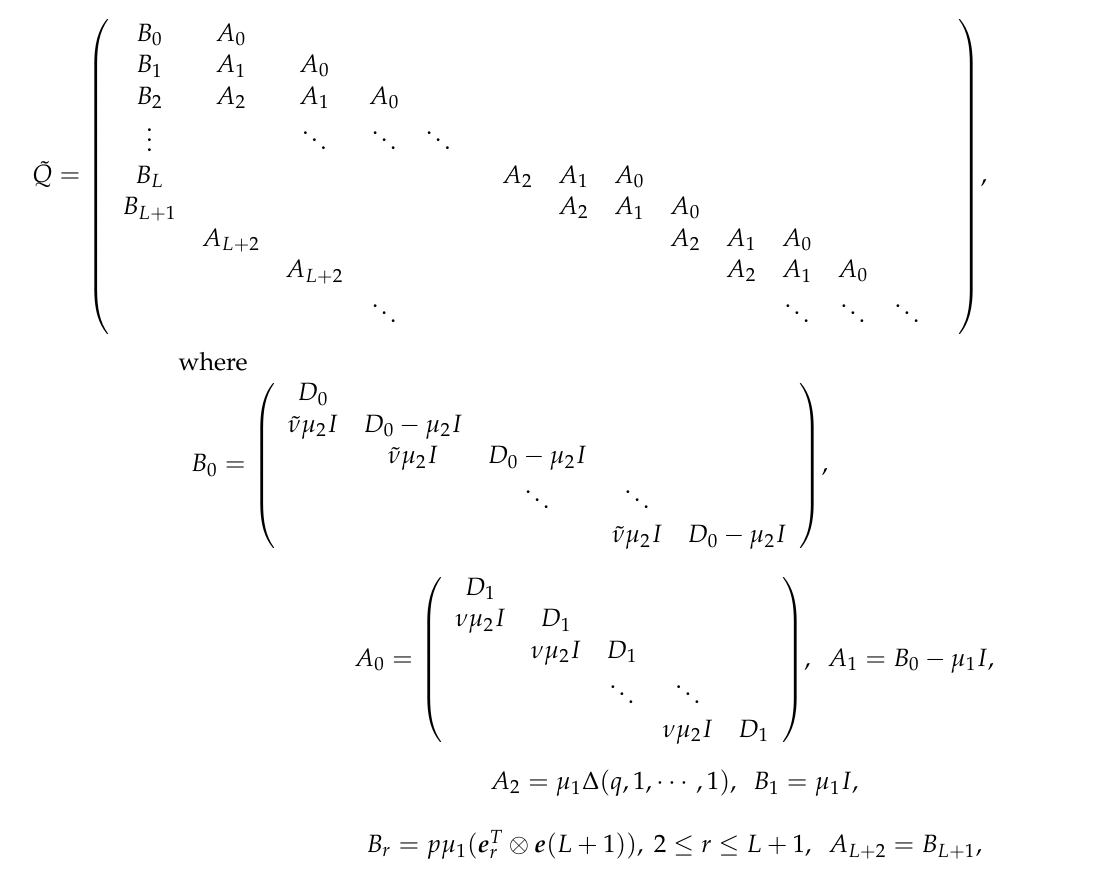
\includegraphics[width=0.9\textwidth]{FcngTm3.png}
    \label{fig:GI-M-1}
\end{figure}

\textsc{Guardare paper, troppo lungo}

\section{Risultati numerici}

In questa sezione, forniamo alcuni esempi illustrativi utilizzando cinque diversi processi di arrivo. Di questi cinque, tre sono processi di rinnovo e due sono processi correlati. In particolare, prendiamo i cinque MAP come:
\begin{itemize}
    \item \textbf{ERL}: Questo è un Erlang di ordine 5 con parametro 2.5 in ciascuno dei 5 stati. Notare che qui abbiamo $\lambda = 0.5, \sigma = 0.899427$ e $\rho_c = 0$.
    \item \textbf{EXP}: Questo è un esponenziale con una frequenza di 0.5. Notare che qui abbiamo $\lambda = 0.5, \sigma = 2$ e $\rho_c = 0$.
    \item \textbf{HEX}: Questa è una distribuzione iper-esponenziale con una probabilità di mixing data da (0.5, 0.3, 0.15, 0.04, 0.01) con i corrispondenti tassi della distribuzione esponenziale pari a (1.09, 0.545, 0.2725, 0.13625, 0.068125). Qui abbiamo $\lambda = 0.5, \sigma = 3.3942$ e $\rho_c = 0$.
\end{itemize}
I due processi correlati, negativo e positivo, sono i seguenti:
\begin{itemize}
    \item \textbf{NCR}: Questo è un MAP negativamente correlato, con matrici di rappresentazione date da:
    \begin{figure}[h!]
        \centering
        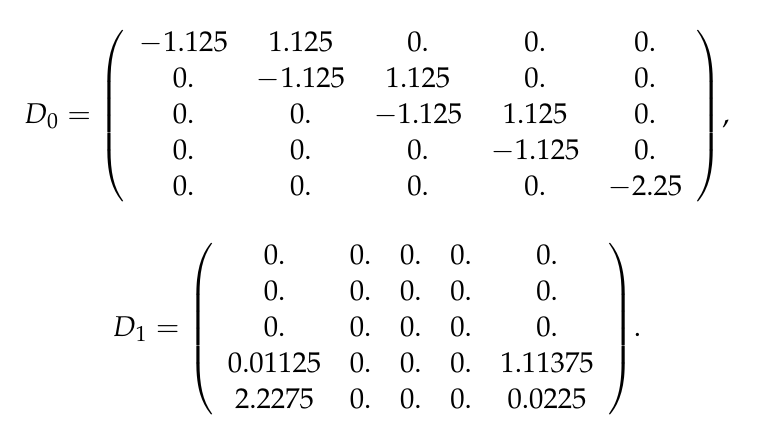
\includegraphics[width=0.6\textwidth]{GYJt39w.png}
        \label{fig:NCR}
    \end{figure}
    dove abbiamo $\lambda = 0.5, \sigma = 2.02454$ e $\rho_c =  -0.57855$.
    \item \textbf{PCR}: Questo è un MAP positivamente correlato, con matrici di rappresentazione date da:
    \begin{figure}
        \centering
        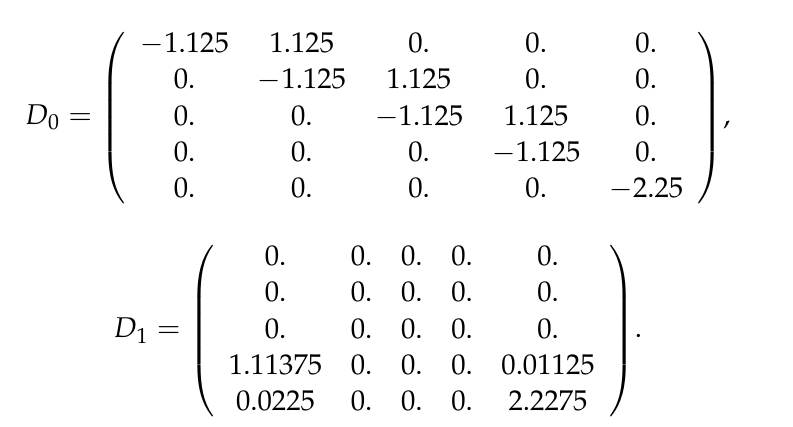
\includegraphics[width=0.6\textwidth]{GFF6s3y.png}
        \label{fig:PCR}
    \end{figure}
    dove abbiamo $\lambda = 0.5, \sigma = 2.02454$ e $\rho_c = 0.57855$.
\end{itemize}
Guardando le cinque MAP sopra riportate, è evidente che sono tutte qualitativamente diverse. È importante sottolineare che il processo di arrivo denominato PCR è ideale per situazioni in cui gli arrivi dei clienti sono altamente irregolari, con periodi alternati di congestione e di scarsità del sistema. Tali arrivi sono comuni nella pratica, specialmente nelle telecomunicazioni e nelle industrie dei servizi. È importante notare, inoltre, che il processo di arrivo denominato HEX è noto per presentare un comportamento irregolare simile nel senso che gli arrivi con tempi tra di essi più brevi sono separati da tempi più lunghi. Tuttavia, la differenza tra questi due processi sta nella correlazione positiva presente nel processo PCR. L'impatto di questa correlazione positiva, così come dell'elevata variabilità nei tempi tra gli arrivi, come nei due processi sopra citati, è stato ben documentato in letteratura (vedi, ad esempio, riferimenti [29,30]). Discutiamo tre esempi numerici rappresentativi e illustrativi per evidenziare la natura qualitativa del modello in studio.

\subsection{Primo esempio numerico}
Qui discutiamo l'impatto del parametro L su alcune misure di performance del sistema selezionate per tutte e cinque le MAP. Innanzitutto, fissiamo $\mu_1=1$, $\mu_2=0.5$, $q=0.5$, e $\nu=0.4$, e variamo $L$ da 1 a 30.

\begin{figure}[h]
    \centering
    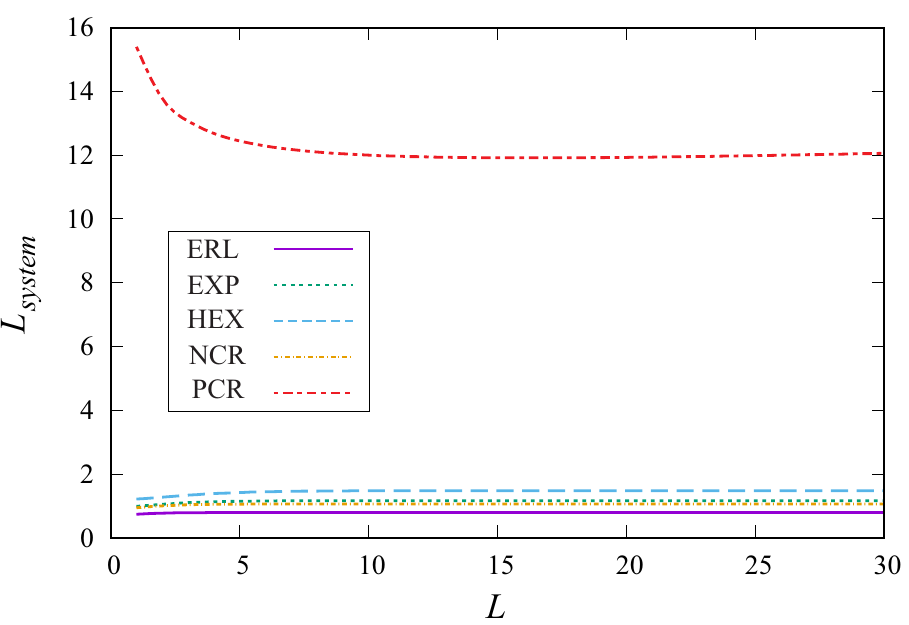
\includegraphics[width=0.7\textwidth]{gtHnIzQ.png}
    \caption{Impact of L on the average number of customers in the system $L_{system}$ for different MAPs.}
    \label{fig:1}
\end{figure}
La Figura \ref{fig:1} illustra chiaramente l'effetto dell'irregolarità nel processo di arrivo, ovvero PCR. Il numero medio di clienti nel sistema nel caso di PCR è molte volte maggiore rispetto agli altri MAPs. Vale la pena sottolineare che per i primi quattro MAPs, la misura $L_\text{system}$ è una funzione non decrescente di $L$, mentre per PCR si osserva un trend non crescente. Ciò spiega il ruolo della correlazione, soprattutto positiva, e non dovrebbe essere ignorato. Inoltre, un valore elevato di L indica che quando un server secondario viene reclutato, verranno assegnati più clienti e, a causa della lentezza del server secondario (rispetto al server principale), c'è una alta probabilità, soprattutto per i casi dei primi quattro MAPs, che il sistema abbia in media più clienti nel sistema. Similmente a quanto noto nella coda classica, ovvero il numero medio nel sistema aumenta con l'aumento della variabilità nei tempi di arrivo tra gli arrivi di rinnovo, vediamo che questo comportamento si verifica anche qui nei primi tre MAPs, che corrispondono agli arrivi di rinnovo. \vspace{0.4cm}

\noindent Tuttavia, per quanto riguarda gli arrivi PCR, osserviamo un trend interessante ma opposto, ovvero un trend decrescente. Questo può essere intuitivamente spiegato come segue. Innanzitutto, si osserva che il sistema L ha un valore massimo di 15.3983 quando $L = 1$, il che può essere spiegato utilizzando il fatto che, quando $L = 1$, i server secondari lasciano il sistema dopo aver servito un solo cliente; con una probabilità del solo 0.5 di essere reclutati, la coda tende ad accumularsi rapidamente. Aumentando L, i server secondari sono maggiormente coinvolti nella pulizia della coda, soprattutto quando gli arrivi avvengono a sprazzi, e quindi $L_\text{system}$ diminuisce. Raggiunge un valore minimo di 11.9757 quando $L = 16$ e poi inizia ad aumentare a causa della mancata possibilità di essere serviti dal server principale. Per $L = 30, L_\text{system} = 12.0605$ \vspace{0.4cm}

\begin{figure}[h]
    \centering
    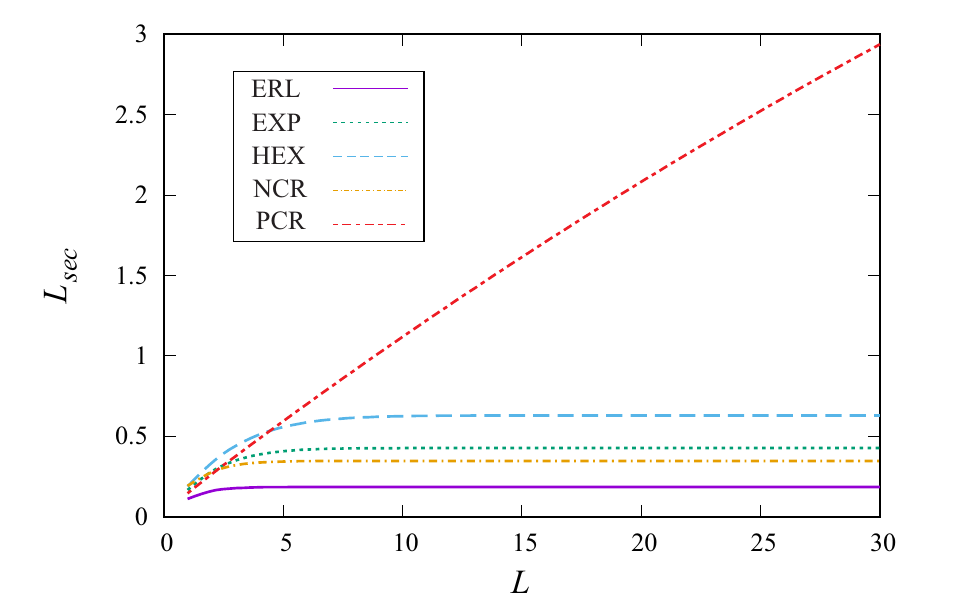
\includegraphics[width=0.8\textwidth]{Tcjl81t.png}
    \caption{ Dependence of the average number of customers with the secondary server L sec on the
    parameter L for different MAPs.}
    \label{fig:2}
\end{figure}

\noindent La Figura \ref{fig:2} mostra il comportamento della media del numero di clienti con il server secondario $L_{\mathrm{sec}}$.

\clearpage
\begin{figure}[h]
    \centering
    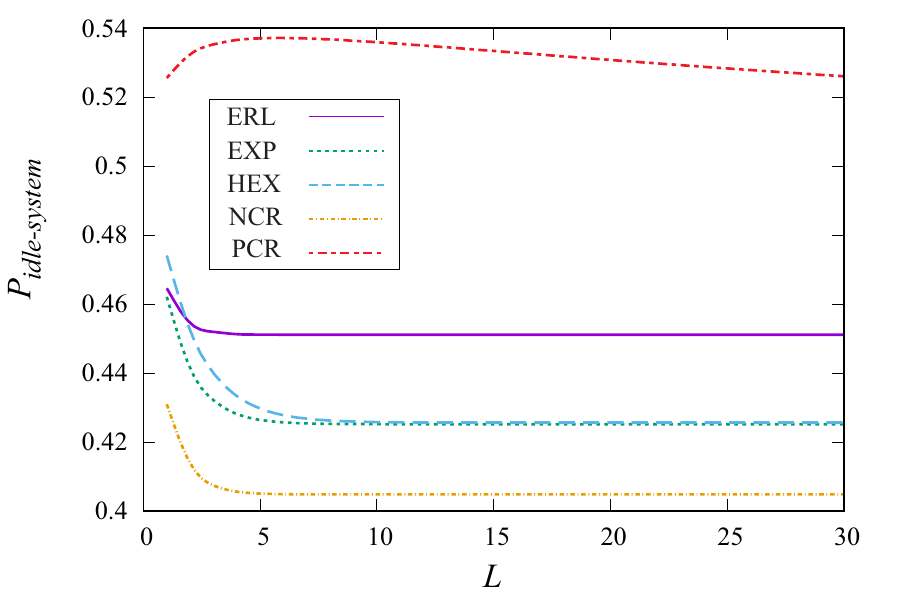
\includegraphics[width=0.8\textwidth]{pSUZiNk.png}
    \caption{ Dependence of the probability $P_{\mathrm{idle-system}}$ that the system is idle at an arbitrary moment on the parameter L for different MAPs}
    \label{fig:3}
\end{figure}

La Figura \ref{fig:3} illustra il comportamento della probabilità,  $P_{\mathrm{idle-system}}$, che il sistema sia inattivo in un momento arbitrario. Questa figura corrisponde alla Figura \ref{fig:1} su due aspetti. Il primo è che mostra anche una grande differenza nella misura quando viene confrontata con vari MAPs. Quando si cerca di trovare un valore ottimale di L, è evidente che conta quale misura viene scelta come funzione obiettivo e il tipo di MAPs utilizzato quando tutti gli altri parametri sono fissati. Ad esempio, se si considera il processo di arrivo PCR, il valore ottimale di L è 16 se si cerca di minimizzare $L_{\mathrm{system}}$. Tuttavia, se la misura  $P_{\mathrm{idle-system}}$ è l'obiettivo del problema di ottimizzazione, allora $L = $6 produce il valore più grande per questa misura. \vspace{0.4cm}

\begin{figure}[h]
    \centering
    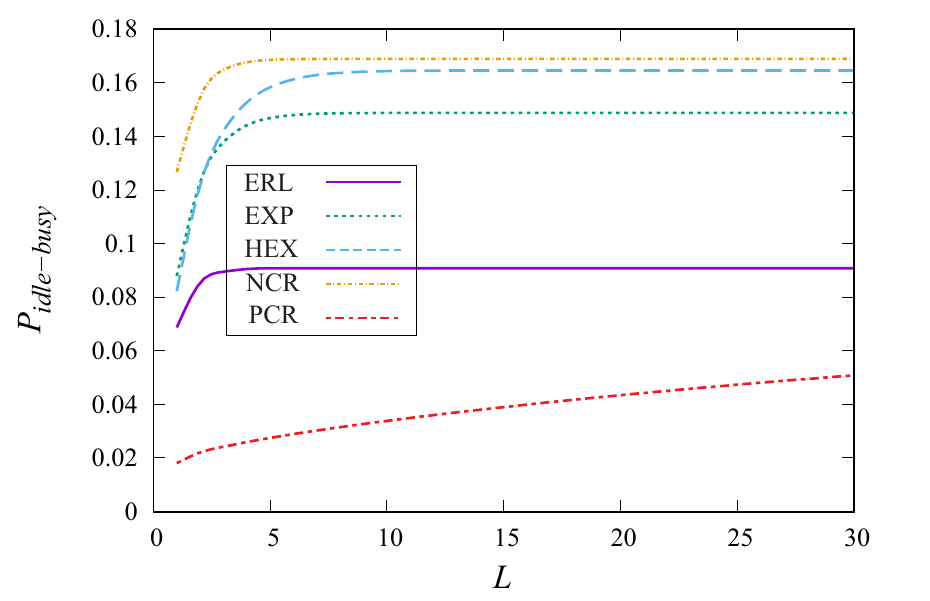
\includegraphics[width=0.8\textwidth]{VrxLKYI.png}
    \caption{ Dependence of the probability $P_{\mathrm{idle-busy}}$ that the main server is idle while the secondary server is busy on the parameter L for different MAPs}
    \label{fig:4}
\end{figure}

\begin{figure}
    \centering
    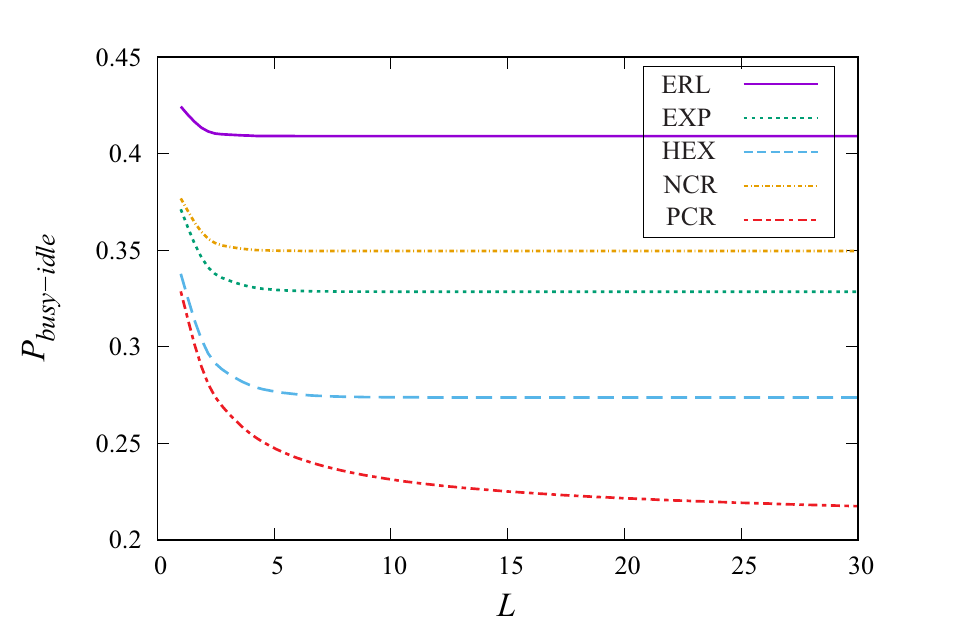
\includegraphics[width=0.8\textwidth]{EZp90oP.png}
    \caption{Dependence of the probability $P_{\mathrm{busy-idle}}$ that the main server is busy while the secondary server is idle on the parameter L for different MAPs.}
    \label{fig:5}
\end{figure}

Le Figure \ref{fig:4} e \ref{fig:5} illustrano il comportamento delle probabilità $P_{\mathrm{idle-busy}}$ e  $P_{\mathrm{busy-idle}}$, che corrispondono rispettivamente al momento in cui il server principale è inattivo con il server secondario occupato, e al momento in cui il server principale è occupato con il server secondario inattivo, in un momento arbitrario. Mentre la prima probabilità aumenta all'aumentare di L, la seconda probabilità diminuisce. Da queste figure, si possono notare le differenze essenziali in queste probabilità in vari scenari.

\clearpage

\subsection{Secondo esempio numerico}
Lo scopo di questo esempio è di indagare l'impatto dei parametri $q$ (ricorda che questo è la probabilità che un cliente servito si rifiuti di agire come server secondario) e $\nu$ (questa è la probabilità che un cliente servito da un server secondario sia insoddisfatto e torni al sistema). Fissiamo il valore di $L$ a $10$ (punto medio tra i due valori ottimali menzionati nel primo esempio). Fissiamo anche i tassi di servizio come $\mu_1 = 1$ e $\mu_2 = 0.5$ e indaghiamo la dipendenza di diverse misure di prestazione dalle probabilità $q$ e $\nu$. Variamo i valori di queste probabilità da $0$ a $1$ con passo $0.05$. Si noti che il valore $q = 1$ corrisponde al classico sistema MAP/M/1 con il tasso di servizio $\mu_1$. \vspace{0.4cm}.

\noindent In questo esempio ci concentriamo sul processo di arrivo etichettato come PCR, la cui scelta è basata sul comportamento di questo processo sulle misure evidenziato nel primo esempio illustrativo. Dalla Figura \ref{fig:6}, che mostra la dipendenza del numero medio di clienti nel sistema $L_\mathrm{system}$ dai parametri $q$ e $\nu$, deduciamo diverse osservazioni interessanti.

\begin{figure}[h]
    \centering
    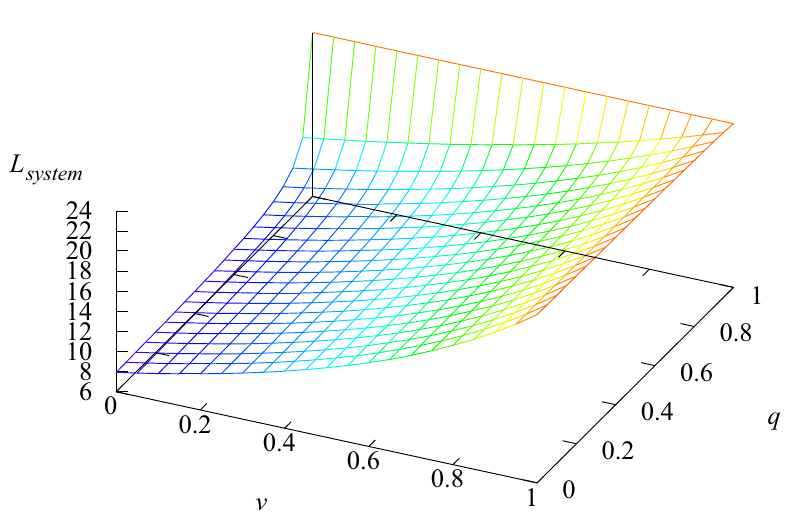
\includegraphics[width=0.7\textwidth]{qUQVrEZ.png}
    \caption{Dependence of the average number of customers in the system $L_\mathrm{system}$ on the parameters q and $\nu$.}
    \label{fig:6}
\end{figure}

Il valore di $L_\mathrm{system}$ è minimo con un valore di $7,9328$ quando il cliente servito è sempre disponibile per essere reclutato (quando il sistema ne ha bisogno) e quando il cliente che riceve il servizio da un server secondario è sempre soddisfatto. Il valore minimo si ottiene quando $q = 0$ e $\nu = 0$. Questa misura aumenta quando aumenta $q$ o $\nu$, e il tasso di aumento diventa più elevato quando uno o entrambi si avvicinano al valore 1. Quando $q = 1$, il sistema si trasforma nel corrispondente modello di coda MAP/M/1 classico e in un sistema senza l'uso del server secondario, e $L_\mathrm{system} = 22,30425$ per tutti i valori di $\nu$ (come è evidente). Quando $q = 0$, che corrisponde al caso in cui un cliente servito viene sempre reclutato (quando necessario), anche quando la probabilità di insoddisfazione è alta ($\nu = 0,5$), il valore di $L_\mathrm{system}$ è pari a $12,91247$. Pertanto, l'uso di un server secondario riduce essenzialmente il numero medio di clienti nel sistema di più del $40\%$. Inoltre, abbiamo cercato il punto di interruzione, diciamo $\nu^*$, per una percentuale di insoddisfazione tale per cui il modello classico di coda è migliore del modello proposto qui. Per i parametri di questo esempio, il punto di interruzione è $\nu^* \sim 0,985$, nel senso che la percentuale di insoddisfazione deve essere superiore al $98,5\%$ affinché il modello classico funzioni meglio. \vspace{0.4cm}

\begin{figure}[h]
    \centering
    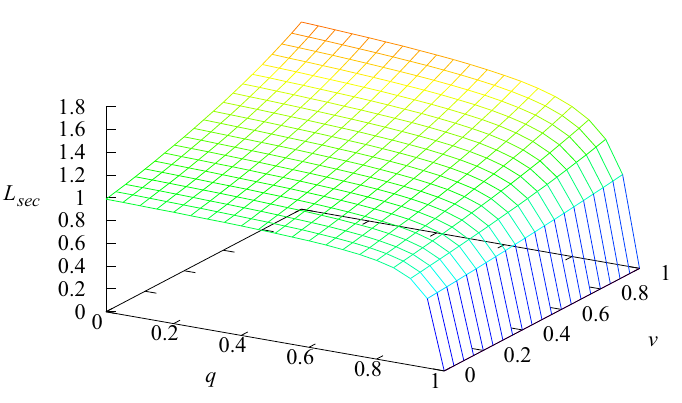
\includegraphics[width=0.6\textwidth]{0uFWo7C.png}
    \caption{Dependence of the average number of customers with the secondary server $L_\mathrm{sec}$ on the parameters $q$ and $\nu$}
    \label{fig:7}
\end{figure}

Per testare ulteriormente l'importo della riduzione nel numero medio, abbiamo aumentato $\lambda$ del $50\%$ a $\lambda = 0.75$. Mantenendo tutti gli altri parametri (ad eccezione della normalizzazione dei parametri del processo di arrivo per ottenere questo specifico $\lambda$) gli stessi, abbiamo ottenuto una percentuale di riduzione superiore al $52,8\%$. Pertanto, un aumento del carico del sistema beneficerà notevolmente dell'avere un server secondario per aiutare il sistema anche con un tasso di insoddisfazione del cliente del $50\%$ con questo server secondario.
La figura \ref{fig:7} mostra la dipendenza del numero medio di clienti con il server secondario $L_\mathrm{sec}$ dai parametri $q$ e $\nu$. Questa probabilità diminuisce significativamente quando $q$ si avvicina a $1$ e quando i clienti sono raramente reclutati per diventare server secondari. $L_\mathrm{sec}$ ha il valore massimo quando $q$ è uguale a zero, ovvero tutti i clienti vengono reclutati (quando necessario) per diventare server secondari, e quando $\nu$ è vicino a 1. Ovviamente, in quest'ultimo caso, quasi tutti i clienti serviti da un server secondario devono essere rimandati al sistema a causa della loro insoddisfazione. Questo spiega la creazione di ulteriore lavoro per il sistema e dovrebbe essere scoraggiato ricorrendo alla coda classica anziché reclutare server secondari "scarsi". Vale la pena sottolineare che un sistema del genere (scadente) può riflettersi negativamente sul sistema stesso per la fornitura di servizi che non possono essere replicati da altri clienti serviti.

\begin{figure}[h!]
    \centering
    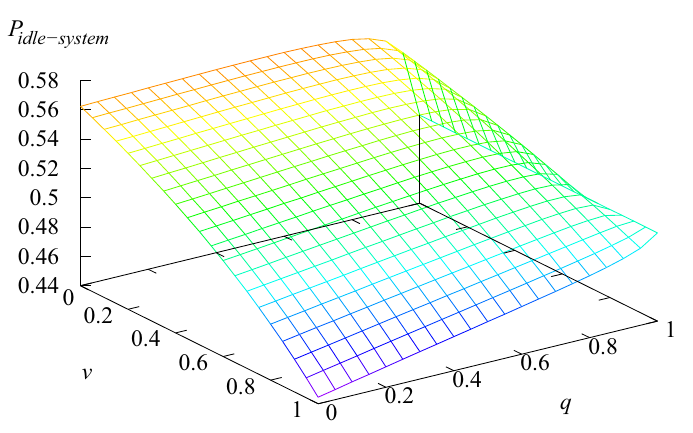
\includegraphics[width=0.6\textwidth]{3zlg6uj.png}
    \caption{Dependence of the probability $P_\mathrm{idle-system}$ that the system is idle at an arbitrary moment on the parameters $q$ and $\nu$.}
    \label{fig:8}
\end{figure}

Nella Figura \ref{fig:8}, è mostrato il comportamento della probabilità $P_\mathrm{idle-system}$ che il sistema è inattivo in un momento arbitrario come funzione di $q$ e $\nu$. Questa probabilità ha il valore minimo di $0.4445$ quando $\nu = 1$ e $q = 0$, il che è intuitivamente chiaro, poiché dover servire nuovamente i clienti dopo aver passato attraverso un server secondario mette un carico sul sistema. La probabilità che $P_\mathrm{idle-system}$ aumenta quando $q$ aumenta e/o $\nu$ diminuisce: il valore massimo $0.5652$ di questa probabilità si ottiene quando $q = 0.65$ e $\nu = 0$. Nel corrispondente sistema MAP/M/1 classico, questa misura è $P_\mathrm{idle-system} = 0.5$.

\vspace{0.4cm}

\noindent \textsc{Altre cose da dire su questo esempio numerico che secondo me si possono saltare. Tornare dopo}

\clearpage
\subsection{Esempio numerico 3}

In questo ultimo esempio, analizziamo l'impatto della variazione dei tassi di servizio $\mu_1$ e $\mu_2$ quando tutti gli altri parametri sono fissati. A tal fine, fissiamo $L = 10$, $q = 0.5$, $\nu = 0.4$ e $\lambda = 0.5$. I tassi $\mu_1$ e $\mu_2$ vengono variati da $0.25$ a $2.0$ con incrementi di $0.05$. È importante menzionare che, per soddisfare la condizione di ergodicità (vedi Equazione \ref{eq:ergodicity}), limitiamo ulteriormente il valore di $\mu_2$ quando $\mu_1$ è piccolo. In particolare, quando $\mu_1 = 0.25$, il valore minimo del tasso $\mu_2$ (con il passo sopra descritto di $0.05$) è scelto in modo tale da non essere inferiore a $0.65$. Quando $\mu_1 = 0.3$, il tasso $\mu_2$ è scelto in modo tale da non essere inferiore a $0.45$. Quando $\mu_1 = 0.35$, il tasso $\mu_2$ è scelto in modo tale da non essere inferiore a $0.3$. Solo per $\mu_1 \geq 0.4$, il valore di $\mu_2$ può essere variato da $0.25$, come originariamente indicato.


Con le sopra descritte restrizioni sulla scelta di $\mu_1$ e $\mu_2$, mostriamo nelle Figure \ref{fig:9} e \ref{fig:10} la dipendenza della misura $L_{\text{system}}$ da $\mu_1$ e $\mu_2$. Nella Figura \ref{fig:9}, gran parte della superficie che mostra la dipendenza appare piatta. Ciò è dovuto al fatto che, per molte combinazioni dei valori dei parametri con un piccolo tasso $\mu_1$, la condizione di ergodicità viene violata e la misura $L_{\text{system}}$ diventa molto grande. Pertanto, nella Figura \ref{fig:10}, la dipendenza di $L_{\text{system}}$ da $\mu_1$ e $\mu_2$ è mostrata solo per valori non piccoli di $\mu_1$. Chiaramente, si può notare una tendenza decrescente, poiché $L_{\text{system}}$ diminuisce rapidamente quando $\mu_1$ aumenta per $\mu_2$ fissato e viceversa.

\begin{figure}[h]
    \centering
    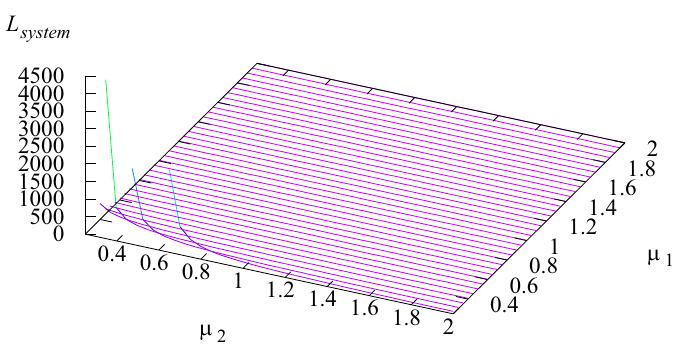
\includegraphics[width=0.6\textwidth]{9LBRzWR.png}
    \caption{Dependence of the average number of customers in the system $L_\mathrm{system}$ on the parameters
    $\mu_1$ and $\mu_2$}
    \label{fig:9}
\end{figure}

\begin{figure}[h]
    \centering
    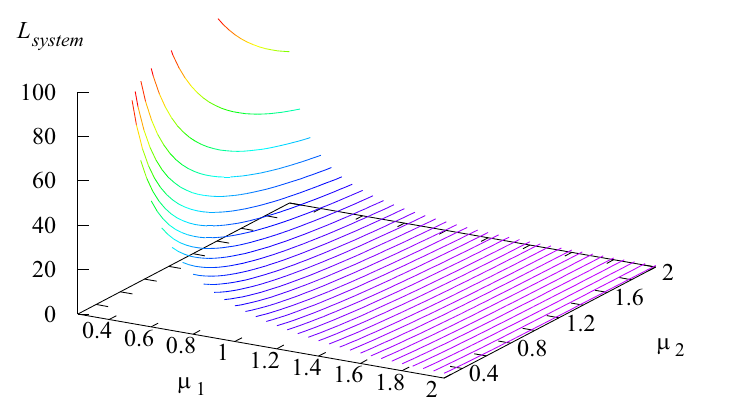
\includegraphics[width=0.6\textwidth]{CBOSr9C.png}
    \caption{Dependence of the average number of customers in the system $L_\mathrm{system}$ on the parameters
    $\mu_1$ and $\mu_2$.}
    \label{fig:10}
\end{figure}

La Figura \ref{fig:11} mostra il comportamento del numero medio di clienti con il server
secondario $L_\mathrm{sec}$. Il valore di $L_\mathrm{sec}$ è massimizzato con un valore di circa 5 quando $\mu_1$ e $\mu_2$ sono piccoli. Questo è intuitivamente chiaro poiché per valori piccoli di $\mu_1$ e $\mu_2$, la condizione di ergodicità è vicina a essere violata, causando un alto tasso di reclutamento per i server secondari che, molto probabilmente prima di lasciare il sistema, serviranno un gruppo di dimensione $L = 10$. Pertanto, il numero medio di clienti in servizio in un momento arbitrario è di circa 5. Con un aumento di $\mu_1$ e $\mu_2$, il valore di $L_\mathrm{sec}$ diminuisce come ci si aspetterebbe. Per valori piccoli di $\mu_1$, la diminuzione è significativa all'aumentare di $\mu_2$; per valori più grandi di $\mu_1$, notiamo un tasso insignificante di diminuzione in $L_\mathrm{sec}$ con un aumento di $\mu_2$.

\begin{figure}[h]
    \centering
    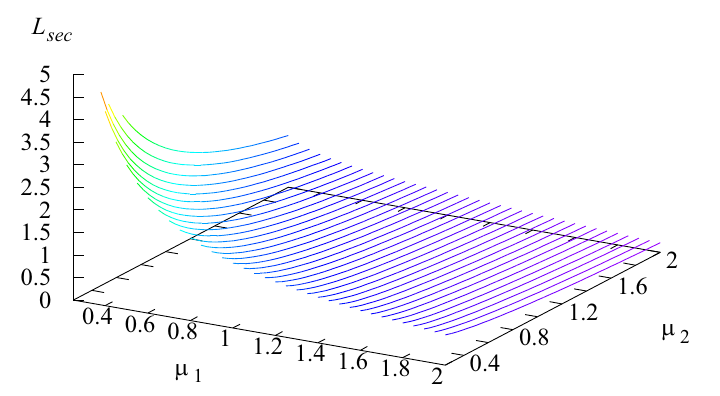
\includegraphics[width=0.6\textwidth]{R1VGHAR.png}
    \caption{Dependence of the average number of customers with the secondary server L sec on the
    parameters $\mu_1$ and $\mu_2$.}
    \label{fig:11}
\end{figure}

\vspace{0.4cm}

\noindent \textsc{Altre cose da dire su questo esempio numerico che secondo me si possono saltare. Tornare dopo}

\clearpage
\section{Conclusioni}
In questo articolo, è stato analizzato un sistema di coda in cui c'è la possibilità di reclutare un cliente già servito come server secondario per aiutare il server principale assegnando un gruppo di clienti in attesa. Il processo di arrivo è stato modellizzato utilizzando un processo di punto Markoviano versatile, MAP. È stata presa in considerazione la possibilità di insoddisfazione dei clienti con il servizio fornito dal server secondario, causando il ritorno di quei clienti nel sistema. È stata implementata l'analisi dello stato stazionario della catena di Markov multidimensionale che descrive il comportamento del sistema e sono stati presentati risultati numerici illustrativi potenzialmente utili per prendere decisioni manageriali.
Il modello studiato in questo articolo può essere generalizzato in diversi modi. Ad esempio,
\begin{enumerate}
    \item il servizio fornito dal server secondario può essere effettuato in gruppi;
    \item  rilassare l'ipotesi di avere solo un server secondario a più di uno e vedere l'impatto dell'aumento a, diciamo, 2;
    \item  utilizzare servizi di tipo fase-possibilmente con rappresentazioni diverse per il server principale e secondario;
    \item incorporare l'impazienza dei clienti sia nei buffer principali che secondari;
    \item  implementare un processo di reclutamento in base alla lunghezza della coda osservata basato su una politica di controllo di tipo soglia;
    \item  consentire arrivi di gruppo; e infine
    \item  incorporare la possibilità di reclutare molti server secondari con due tipi di clienti in modo che solo un tipo possa agire come server secondario.
\end{enumerate}

\end{document}
